\section{Approach}
\label{sec:approach}

We seek to facilitate the creative coloring process by automatically suggesting pattern colorings. In doing so, we must keep in mind that users may or may not have a target coloring style in mind. In addition, aesthetic taste varies across users and can depend on the situation. Thus, an effective color support system should both output a variety of appealing colorings as well as provide controls for personalizing suggestions to a preferred coloring style.

Our system takes as input a pattern template and outputs suggested colorings for that template. A pattern template specifies which \emph{segments}, or connected components, in an image can be colored in and which segments must map to the same color. For example, an image of a flower on a background may have a template that specifies all petals of the flower must be the same color, and all background segments must be the same color. We refer to the set of segments that map to the same color as a \emph{color group}. Figure~\ref{fig:teaser} shows an example of a pattern template visualized in grayscale, where each lightness level identifies a different color group. This template representation is relatively easy to author from images composed of segments, such as web designs, 3D renderings, and line drawings.

To generate attractive pattern colorings, a reasonable first step is to enforce that colors are by some definition `compatible' with one another. Figure~\ref{fig:ColorCompatOnly} shows several patterns whose colors receive a high score under the color compatibility model of O'Donovan et al.~\shortcite{ODonovan}. While these high-scoring colorings use attractive colors and exhibit a great degree of diversity, they also display several problems. Some background regions may be oversaturated, coming across as too `loud.' Several foreground regions have insufficient contrast with the pattern background, causing them to blend uncomfortably into the background.

\begin{figure}[htb]
\centering
%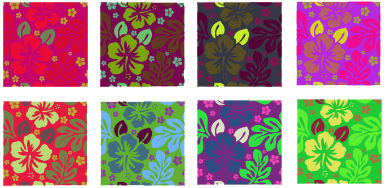
\includegraphics[width=\columnwidth]{figs/colorCompatOnly.png}
\begin{tabular}{cccc}

\includegraphics[width=.2\columnwidth]{figs/colorCompat/r_0_0_3-75}&

\includegraphics[width=.2\columnwidth]{figs/colorCompat/r_0_1_3-32}&
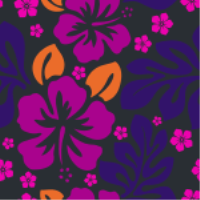
\includegraphics[width=.2\columnwidth]{figs/colorCompat/r_0_2_3-67}&
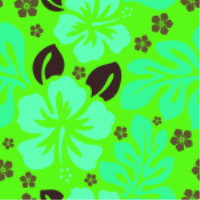
\includegraphics[width=.2\columnwidth]{figs/colorCompat/r_0_3_3-70}\\
3.75&3.32&3.67&3.70\vspace{0.5em}\\

\includegraphics[width=.2\columnwidth]{figs/colorCompat/r_1_0_3-74}&

\includegraphics[width=.2\columnwidth]{figs/colorCompat/r_1_1_3-42}&
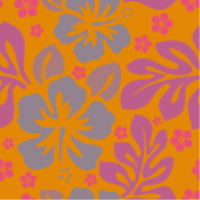
\includegraphics[width=.2\columnwidth]{figs/colorCompat/r_1_2_3-66}&
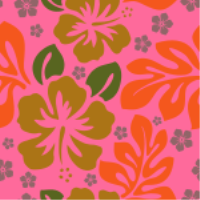
\includegraphics[width=.2\columnwidth]{figs/colorCompat/r_1_3_3-39}\\
3.74&3.42&3.66&3.39\\
\end{tabular}
\caption{Patterns whose colors receive high scores under the color compatibility model of O'Donovan et al.~\shortcite{ODonovan}. The score assigned by the O'Donovan model is shown beneath each pattern; a typical pattern scores between 2 and 4. Many results exhibit problems such as adjacent equi-luminant regions and excessively saturated backgrounds.}
\label{fig:ColorCompatOnly}
\end{figure}

To overcome these problems, we turn to examples of well-colored patterns for help. If we inspect color groups that are large, highly connected, and spread across the entire pattern---indicative features of a background---we can see how saturated they are. This knowledge should prevent us from using excessively `loud' background colors. If we examine the contrast between adjacent pattern regions, we might find that large foreground regions have high contrast with the background but less contrast with thin borders and outlines. Enforcing these same properties in our own colorings should lead to better results.

Consequently, the approach we take to pattern coloring is \emph{data-driven}: given a dataset of example patterns, we learn distributions over color properties such as saturation, lightness, and contrast for individual regions and for adjacent regions. We predict these distributions using discriminative spatial features of the pattern, such as the size and shape of different regions. Finally, we use the predicted distributions to score the goodness of pattern colorings.

In the next sections, we introduce the dataset of patterns we use for our experiments (Section~\ref{sec:dataset}). Next, we describe the \emph{unary color functions} that we use to score the colors of indvidual pattern regions (Section~\ref{sec:unary}), as well the \emph{pairwise color functions} that score the colors of adjacent regions (Section~\ref{sec:binary}). While color compatibility alone does not predict good pattern colorings, it helps to enforce global consistency between colors, and our approach makes use of this ability (Section~\ref{sec:colorCompat}).

We then show how these three different types of scoring functions---\emph{unary}, \emph{pairwise}, and \emph{global}---can be combined into one unified model using the framework of probabilistic factor graphs (Section~\ref{sec:model}). The resulting model is very flexible: we can sample from it to generate a variety of new coloring suggestions, train it on different example sets to capture different coloring styles, and add additional constraints to it to support different usage scenarios (Section~\ref{sec:results}).
